\section{Theoretische Grundlagen}

In diesem Kapitel werden die theoretischen Grundlagen erläutert, die für das Verständnis der entwickelten Middleware-Architektur erforderlich sind. Zunächst werden die verwendeten SAP-Technologien vorgestellt (Abschnitt~2.1--2.3), anschließend REST und Cloud Computing (Abschnitt~2.4--2.5), dann relevante Architekturmuster (Abschnitt~2.6) und abschließend die Microsoft Graph API für den SharePoint-Zugriff (Abschnitt~2.7).

\subsection{SAP Business Technology Platform}

Die SAP \gls{btp} ist die zentrale Entwicklungs- und Integrationsplattform von SAP für Cloud-Anwendungen \citep{sap2024btp}. Sie vereint Datenbank-, Analyse-, Integrations- und Entwicklungsfunktionen in einer einheitlichen Umgebung. Die Plattform gliedert sich in vier zentrale Bereiche: Database \& Data Management (SAP HANA Cloud, Data Intelligence), Analytics (SAP Analytics Cloud, Embedded Analytics), Application Development \& Integration (CAP, Integration Suite, API Management) sowie Intelligent Technologies (AI, Machine Learning, IoT). Für die Entwicklung von Enterprise-Anwendungen stellt die BTP verschiedene Laufzeitumgebungen bereit, darunter Cloud Foundry, Kyma (Kubernetes-basiert) und ABAP Environment \citep{erl2013}.

\subsubsection{Cloud Foundry Environment}

Cloud Foundry ist eine Open-Source-Platform-as-a-Service (PaaS), die SAP als primäre Laufzeitumgebung auf der BTP anbietet \citep{cloudfoundry2024}. Sie ermöglicht das Deployment von Anwendungen in verschiedenen Programmiersprachen (Node.js, Java, Python, Go) ohne manuelle Infrastrukturverwaltung.

Die wesentlichen Konzepte von Cloud Foundry umfassen Organizations und Spaces als hierarchische Struktur zur Mandantentrennung und Umgebungsverwaltung (Dev, Test, Prod), Buildpacks zur automatischen Erkennung und Kompilierung der Anwendung basierend auf der Programmiersprache, Services als verwaltete Dienste (Datenbanken, Message Queues), die an Anwendungen gebunden werden, sowie Routes als URL-Mappings für den externen Zugriff auf Anwendungen.

Das Deployment erfolgt über das Cloud Foundry CLI mit dem Befehl \texttt{cf push}, welcher die Anwendung paketiert, einen Container erstellt und die Instanzen startet. Dieser Ansatz folgt dem \enquote{Cloud Native}-Paradigma, bei dem Anwendungen für die Cloud-Umgebung optimiert werden \citep{davis2019}.

\subsubsection{SAP Cloud ALM}

SAP \gls{calm} ist eine cloudbasierte Lösung für das Application Lifecycle Management \citep{sap2024calm}. Es unterstützt Unternehmen bei der Planung, Implementierung und dem Betrieb von SAP-Lösungen über den gesamten Lebenszyklus hinweg.

Die Kernfunktionen von SAP Cloud ALM umfassen den Bereich Implementation mit Projektplanung, Aufgabenverwaltung und Anforderungsmanagement, Operations für Monitoring und Health Management, Analytics mit Dashboards und KPIs sowie Process Management für Prozessdokumentation und Fit-to-Standard-Workshops.

Für diese Arbeit ist insbesondere der Implementation-Bereich relevant, da hier User Stories und deren Aufwände verwaltet werden. SAP Cloud ALM stellt diese Daten über \gls{odata}-Services bereit, was eine programmatische Integration ermöglicht. Die Verwaltung von Projektbudgets und Aufwänden entspricht dabei den etablierten Praktiken des Projektmanagements \citep{kerzner2017, pmi2021}.

\subsection{SAP Cloud Application Programming Model}

Das \gls{cap} ist ein Framework für die Entwicklung von Enterprise-Anwendungen auf der SAP \gls{btp} \citep{sap2024cap}. Es basiert auf bewährten Open-Source-Technologien und bietet eine einheitliche Programmierabstraktion für verschiedene Datenbanken und Protokolle. Das Framework folgt dem Prinzip \enquote{Convention over Configuration} und reduziert Boilerplate-Code durch deklarative Definitionen.

Die Kernprinzipien von CAP orientieren sich am Domain-Driven Design mit Fokus auf das Domänenmodell statt technischer Details \citep{evans2003}. Datenmodelle und Services werden deklarativ in CDS definiert statt in imperativem Code. Das Framework bietet integrierte Unterstützung für OData, REST und Authentifizierung und abstrahiert über verschiedene Datenbanken (SQLite, HANA, PostgreSQL) im Sinne einer polyglotten Persistenz.

\subsubsection{Core Data Services}

\gls{cds} ist die deklarative Modellierungssprache des \gls{cap} \citep{sap2024cds}. Mit \gls{cds} werden Datenmodelle, Services und Annotationen definiert. Die Sprache ist bewusst einfach gehalten und ähnelt SQL in ihrer Syntax.

\begin{lstlisting}[caption={Beispiel einer CDS-Service-Definition}, label={lst:cds-example}]
service BudgetService @(path: '/api/budget') {
    entity PSPElements {
        key psp      : String(50);
            name     : String(200);
            team     : String(100);
            budgetPT : Decimal(15, 2);
    }

    function getProjects() returns array of String;
    action startSession(project : String) returns { ... };
}
\end{lstlisting}

Zentrale CDS-Konzepte sind Entities als Datenstrukturen mit Schlüsselfeldern und Attributen, Services zur Gruppierung von Entities, die als API exponiert werden, Functions für lesende Operationen (HTTP GET), Actions für schreibende Operationen (HTTP POST) sowie Annotations als Metadaten für UI, Validierung und Autorisierung.

Die Annotation \texttt{@cds.persistence.skip} kennzeichnet Entitäten, die nicht in einer Datenbank persistiert werden, sondern zur Laufzeit aus anderen Quellen generiert werden -- ein zentrales Konzept für die BC Middleware.

\subsubsection{Service-Implementierung in Node.js}

Die Geschäftslogik wird in JavaScript (Node.js) implementiert \citep{nodejs2024}. CAP stellt einen ereignisgesteuerten Ansatz mit Handlern für \gls{crud}-Operationen bereit. Die Ereignisse folgen einem einheitlichen Muster:

\begin{lstlisting}[caption={Event Handler in CAP}, label={lst:event-handler}]
module.exports = class BudgetService extends cds.ApplicationService {
    init() {
        // Handler fuer READ-Operation auf PSPElements
        this.on('READ', 'PSPElements', async (req) => {
            const data = await loadFromExcel();
            return data.pspElements;
        });

        // Handler fuer Custom Action
        this.on('startSession', async (req) => {
            const { project } = req.data;
            const sessionId = createSession(project);
            return { success: true, sessionId, project };
        });

        return super.init();
    }
}
\end{lstlisting}

Die verfügbaren Ereignisse gliedern sich in \texttt{before}-Handler, die vor der Operation ausgeführt werden und typischerweise der Validierung dienen, \texttt{on}-Handler, welche die Standardimplementierung der Operation ersetzen, sowie \texttt{after}-Handler für nachgelagerte Transformationen und Logging.

Dieses Modell ermöglicht eine saubere Trennung zwischen der deklarativen API-Definition in CDS und der imperativen Geschäftslogik in JavaScript.

\subsection{REST und RESTful APIs}

Representational State Transfer (REST) ist ein Architekturstil für verteilte Systeme, der von Roy Fielding in seiner Dissertation definiert wurde \citep{fielding2000}. REST basiert auf sechs Grundprinzipien. Das erste Prinzip ist die strikte Trennung zwischen Client und Server (Client-Server-Architektur), die eine unabhängige Entwicklung und Skalierung beider Komponenten ermöglicht. Die Zustandslosigkeit als zweites Prinzip erfordert, dass jede Anfrage alle zur Verarbeitung notwendigen Informationen enthält -- der Server speichert keinen Client-Zustand zwischen Anfragen. Drittens müssen Antworten als cachebar oder nicht-cachebar gekennzeichnet sein (Cachebarkeit), um die Netzwerkeffizienz zu verbessern. Das vierte Prinzip der einheitlichen Schnittstelle besagt, dass Ressourcen über URIs identifiziert und über standardisierte HTTP-Methoden manipuliert werden. Fünftens kann die Architektur als Schichtensystem aus mehreren für den Client transparenten Schichten bestehen (Load Balancer, Caches, Gateways). Das sechste, optionale Prinzip Code on Demand erlaubt es Servern, ausführbaren Code an Clients zu senden.

Die HTTP-Methoden werden in REST wie folgt verwendet:

\begin{table}[H]
\centering
\caption{HTTP-Methoden in REST}
\label{tab:http-methods}
\begin{tabularx}{\textwidth}{llX}
\toprule
\textbf{Methode} & \textbf{CRUD} & \textbf{Beschreibung} \\
\midrule
GET & Read & Ressource abrufen (idempotent, sicher) \\
POST & Create & Neue Ressource erstellen \\
PUT & Update & Ressource vollständig ersetzen (idempotent) \\
PATCH & Update & Ressource teilweise aktualisieren \\
DELETE & Delete & Ressource löschen (idempotent) \\
\bottomrule
\end{tabularx}
\end{table}

OData baut auf diesen REST-Prinzipien auf und erweitert sie um standardisierte Query-Optionen und Metadaten \citep{oasis2020odata}. Im Vergleich zu anderen API-Stilen bietet REST eine gute Balance zwischen Einfachheit und Ausdrucksstärke, was zu seiner weiten Verbreitung im Enterprise-Umfeld beigetragen hat \citep{lauret2019}.

\subsection{Cloud Computing Grundlagen}

Cloud Computing bezeichnet die bedarfsgerechte Bereitstellung von IT-Ressourcen über das Internet \citep{erl2013}. Das National Institute of Standards and Technology (NIST) definiert in seiner weithin anerkannten Definition fünf wesentliche Charakteristiken \citep{mell2011}: On-Demand Self-Service ermöglicht es Nutzern, Ressourcen automatisch und ohne menschliche Interaktion bereitzustellen. Broad Network Access stellt sicher, dass Dienste über Standardnetzwerke und heterogene Client-Plattformen verfügbar sind. Beim Resource Pooling werden Ressourcen des Anbieters gebündelt und dynamisch mehreren Nutzern zugewiesen (Multi-Tenancy). Rapid Elasticity bezeichnet die Fähigkeit, Kapazitäten schnell und oft automatisch bereitzustellen. Schließlich gewährleistet Measured Service, dass die Ressourcennutzung gemessen, überwacht und transparent abgerechnet wird.

\subsubsection{Service-Modelle}

Cloud-Dienste werden in drei Service-Modelle unterteilt:

\begin{figure}[H]
\centering
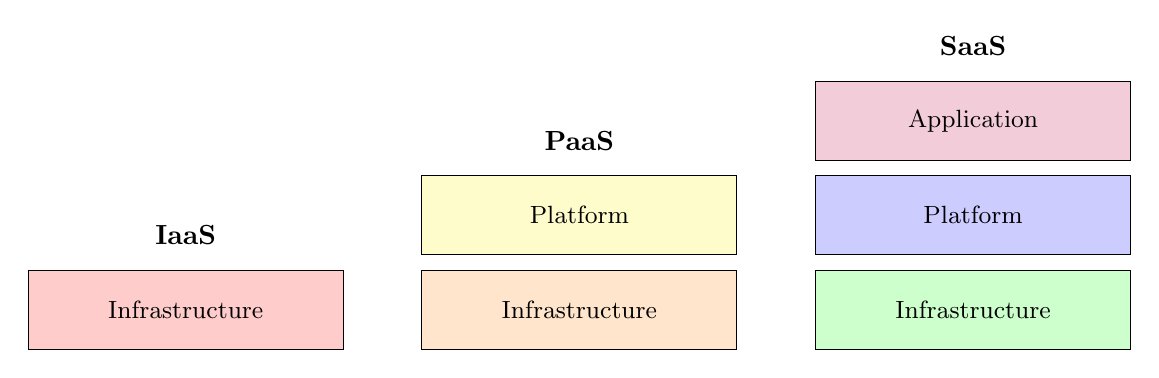
\begin{tikzpicture}[
    layer/.style={rectangle, draw, minimum width=4cm, minimum height=1cm, align=center, font=\small}
]
    % IaaS
    \node[layer, fill=red!20] (iaas-infra) at (0,0) {Infrastructure};
    \node[above] at (0,0.7) {\textbf{IaaS}};

    % PaaS
    \node[layer, fill=orange!20] (paas-infra) at (5,0) {Infrastructure};
    \node[layer, fill=yellow!20] (paas-plat) at (5,1.2) {Platform};
    \node[above] at (5,1.9) {\textbf{PaaS}};

    % SaaS
    \node[layer, fill=green!20] (saas-infra) at (10,0) {Infrastructure};
    \node[layer, fill=blue!20] (saas-plat) at (10,1.2) {Platform};
    \node[layer, fill=purple!20] (saas-app) at (10,2.4) {Application};
    \node[above] at (10,3.1) {\textbf{SaaS}};
\end{tikzpicture}
\caption{Cloud Service-Modelle}
\label{fig:cloud-models}
\end{figure}

Infrastructure as a Service (IaaS) umfasst die Bereitstellung von Rechenleistung, Speicher und Netzwerk, wie beispielsweise Amazon EC2 oder Microsoft Azure VMs. Platform as a Service (PaaS) stellt eine Entwicklungs- und Laufzeitumgebung bereit, bei der der Nutzer lediglich die Anwendung verwaltet -- Beispiele hierfür sind SAP BTP Cloud Foundry und Heroku. Software as a Service (SaaS) bezeichnet die Bereitstellung fertiger Anwendungen wie SAP S/4HANA Cloud oder Microsoft 365.

Wie in Abbildung~\ref{fig:cloud-models} dargestellt, ist die SAP BTP primär ein PaaS-Angebot, das Entwicklern eine Plattform für die Erstellung und den Betrieb von Anwendungen bereitstellt \citep{sap2024btp}.

\subsection{OData Protocol}

Das \gls{odata} ist ein offener Standard für \gls{rest}ful \gls{api}s, der von OASIS standardisiert wurde \citep{oasis2020odata}. Es definiert bewährte Praktiken für den Aufbau und die Nutzung von Web-APIs und wird von SAP als Standard für die Kommunikation zwischen Frontend und Backend verwendet \citep{sap2024odata}.

OData baut auf den Prinzipien von REST auf \citep{fielding2000} und erweitert diese um einheitliche URL-Konventionen für den Ressourcenzugriff, standardisierte Query-Optionen für Filterung, Sortierung und Paginierung, Metadaten-Dokumente zur Selbstbeschreibung der API sowie Batch-Requests für mehrere Operationen in einer Anfrage.

\subsubsection{OData v4}

OData Version 4.01 ist die aktuelle Version des Standards und bietet gegenüber früheren Versionen verbesserte Funktionalität \citep{oasis2020odata}. Die wichtigsten Query-Optionen sind:

\begin{table}[H]
\centering
\caption{OData v4 Query-Optionen}
\label{tab:odata-options}
\begin{tabularx}{\textwidth}{lX}
\toprule
\textbf{Option} & \textbf{Beschreibung} \\
\midrule
\texttt{\$filter} & Filtern von Ergebnissen nach Bedingungen \\
\texttt{\$select} & Auswahl bestimmter Eigenschaften (Projektion) \\
\texttt{\$orderby} & Sortierung nach einer oder mehreren Eigenschaften \\
\texttt{\$top} & Begrenzung der Ergebnismenge \\
\texttt{\$skip} & Überspringen von Ergebnissen (für Paginierung) \\
\texttt{\$expand} & Einbetten verknüpfter Entitäten \\
\texttt{\$count} & Rückgabe der Gesamtanzahl der Ergebnisse \\
\bottomrule
\end{tabularx}
\end{table}

Zusätzlich zu den Query-Optionen definiert OData v4 zwei Arten von benutzerdefinierten Operationen: Functions sind lesende Operationen ohne Seiteneffekte (HTTP GET) -- beispielsweise gibt \texttt{getProjects()} eine Liste verfügbarer Projekte zurück. Actions hingegen sind schreibende Operationen mit potentiellen Seiteneffekten (HTTP POST), etwa \texttt{startSession(project)} zur Erstellung einer neuen Session.

SAP CAP generiert automatisch OData v4-konforme Endpunkte aus den CDS-Service-Definitionen, was die Entwicklung erheblich beschleunigt \citep{sap2024cap}.

\subsection{Architekturmuster}

Die folgenden Architekturmuster bilden das theoretische Fundament für den Entwurf der BC Middleware. Sie ermöglichen eine flexible, wartbare und erweiterbare Architektur \citep{bass2021}.

\subsubsection{Adapter Pattern}

Das Adapter-Pattern ist ein strukturelles Entwurfsmuster, das die Zusammenarbeit von Klassen mit inkompatiblen Schnittstellen ermöglicht \citep{gamma1994}. Es fungiert als Wrapper, der eine Schnittstelle in eine andere übersetzt.

\begin{figure}[H]
\centering
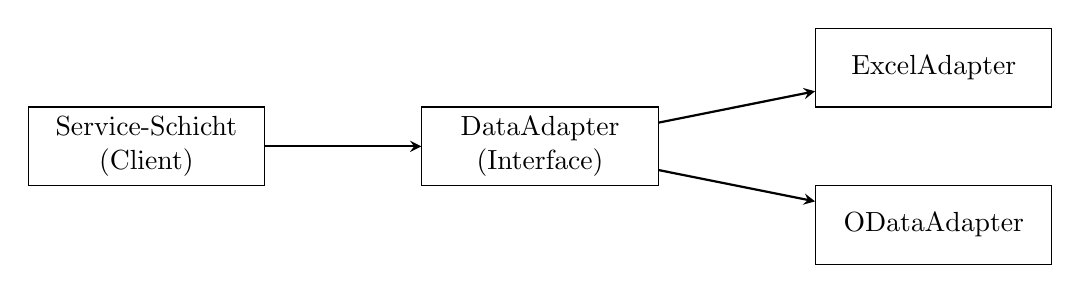
\begin{tikzpicture}[
    box/.style={rectangle, draw, minimum width=3cm, minimum height=1cm, align=center},
    arrow/.style={->, >=stealth, thick}
]
    \node[box] (client) at (0,0) {Service-Schicht\\(Client)};
    \node[box] (interface) at (5,0) {DataAdapter\\(Interface)};
    \node[box] (excel) at (10,1) {ExcelAdapter};
    \node[box] (odata) at (10,-1) {ODataAdapter};

    \draw[arrow] (client) -- (interface);
    \draw[arrow] (interface) -- (excel);
    \draw[arrow] (interface) -- (odata);
\end{tikzpicture}
\caption{Adapter-Pattern für austauschbare Datenquellen}
\label{fig:adapter-pattern}
\end{figure}

Im Kontext dieser Arbeit ermöglicht das Adapter-Pattern den Austausch der Datenquelle (Excel vs. OData-Service), ohne dass die darüberliegende Service-Schicht angepasst werden muss (siehe Abbildung~\ref{fig:adapter-pattern}). Der Adapter übersetzt die spezifische Schnittstelle der Datenquelle (Excel-Datei, REST-API) in ein einheitliches internes Datenmodell.

\subsubsection{Repository Pattern}

Das Repository-Pattern abstrahiert den Datenzugriff und stellt eine einheitliche Schnittstelle für die Geschäftslogik bereit \citep{fowler2002}. Es fungiert als Vermittler zwischen der Domänenschicht und der Datenzugriffsschicht.

Die Vorteile des Repository-Patterns liegen in der Entkopplung der Geschäftslogik von der konkreten Datenquelle, der verbesserten Testbarkeit durch ersetzbare Mock-Objekte, der Zentralisierung der Datenzugriffslogik an einer Stelle sowie der Austauschbarkeit der Implementierung, ohne die Geschäftslogik anpassen zu müssen.

In Kombination mit dem Adapter-Pattern ergibt sich eine Architektur, bei der das Repository die Adapter-Schnittstelle nutzt und die Service-Schicht nur mit dem Repository kommuniziert.

\subsubsection{Schichtenarchitektur}

Die Schichtenarchitektur (engl. Layered Architecture) ist eines der fundamentalsten Architekturmuster in der Softwareentwicklung \citep{bass2021, starke2020}. Sie strukturiert eine Anwendung in horizontale Schichten, wobei jede Schicht eine spezifische Verantwortlichkeit hat und nur mit den direkt benachbarten Schichten kommuniziert.

\begin{figure}[H]
\centering
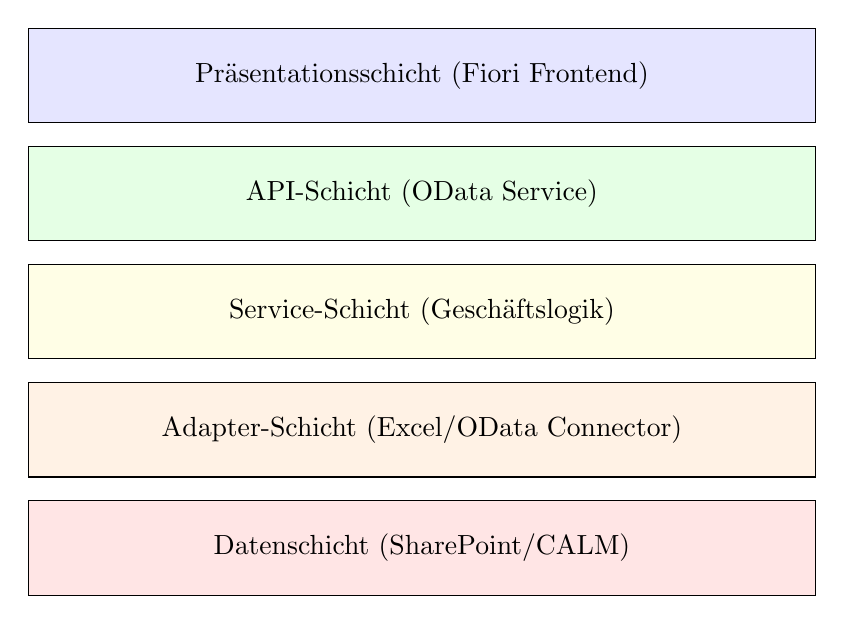
\begin{tikzpicture}[
    layer/.style={rectangle, draw, minimum width=10cm, minimum height=1.2cm, align=center}
]
    \node[layer, fill=blue!10] (pres) at (0,4) {Präsentationsschicht (Fiori Frontend)};
    \node[layer, fill=green!10] (api) at (0,2.5) {API-Schicht (OData Service)};
    \node[layer, fill=yellow!10] (service) at (0,1) {Service-Schicht (Geschäftslogik)};
    \node[layer, fill=orange!10] (adapter) at (0,-0.5) {Adapter-Schicht (Excel/OData Connector)};
    \node[layer, fill=red!10] (data) at (0,-2) {Datenschicht (SharePoint/CALM)};
\end{tikzpicture}
\caption{Schichtenarchitektur der BC Middleware}
\label{fig:layer-architecture}
\end{figure}

Die Vorteile dieser Struktur liegen in der klaren Separation of Concerns, bei der jede Schicht eine definierte Aufgabe hat \citep{sommerville2015}. Änderungen in einer Schicht haben minimale Auswirkungen auf andere Schichten, was die Wartbarkeit erhöht. Zudem können Schichten in anderen Kontexten wiederverwendet und isoliert getestet werden.

\subsection{Microsoft Graph API}

Die Microsoft \gls{graph} ermöglicht den programmgesteuerten Zugriff auf Microsoft 365-Dienste, einschließlich SharePoint und OneDrive \citep{microsoft2024graph}. Sie bietet einen einheitlichen Endpunkt (\texttt{https://graph.microsoft.com}) für den Zugriff auf verschiedene Microsoft-Dienste.

Für die BC Middleware sind insbesondere die SharePoint-Funktionen relevant \citep{microsoft2024sharepoint}: das Lesen von Dateien aus SharePoint-Dokumentbibliotheken, das Schreiben und Aktualisieren von Dateien sowie das Abrufen von Metadaten wie Änderungsdatum und Autor.

\subsubsection{OAuth 2.0 Authentifizierung}

Der Zugriff auf Microsoft Graph erfordert eine Authentifizierung via OAuth 2.0 \citep{microsoft2024oauth}. Für Server-zu-Server-Kommunikation ohne Benutzerinteraktion wird der \enquote{Client Credentials Flow} verwendet. Dabei ist die Anwendung zunächst in Azure Active Directory (Azure AD) registriert und authentifiziert sich mit Client-ID und Client-Secret. Azure AD gibt daraufhin ein Access Token zurück, welches bei allen nachfolgenden API-Anfragen im Authorization-Header mitgesendet wird.

\begin{lstlisting}[caption={Authentifizierung mit Microsoft Graph}, label={lst:ms-auth}]
const { ConfidentialClientApplication } = require('@azure/msal-node');

const msalConfig = {
    auth: {
        clientId: process.env.AZURE_CLIENT_ID,
        clientSecret: process.env.AZURE_CLIENT_SECRET,
        authority: `https://login.microsoftonline.com/${tenantId}`
    }
};

const cca = new ConfidentialClientApplication(msalConfig);
const token = await cca.acquireTokenByClientCredential({
    scopes: ['https://graph.microsoft.com/.default']
});
\end{lstlisting}

Dieser Authentifizierungsmechanismus ermöglicht es der Middleware, ohne manuelle Benutzeranmeldung auf SharePoint-Dateien zuzugreifen -- eine Voraussetzung für den automatisierten Betrieb.
